\documentclass[12pt,a4paper]{article}
\usepackage[utf8]{inputenc}
\usepackage[spanish,es-tabla]{babel}
\usepackage{geometry}
\usepackage{graphicx}
\usepackage{multirow}
\usepackage{tabularx}
\usepackage{mathptmx}
\usepackage{fancyhdr}
\usepackage{array}
\usepackage[table]{xcolor}
\usepackage{titlesec}
\usepackage{setspace}
\usepackage{microtype}
\usepackage{lastpage}
\usepackage{booktabs}
\usepackage{enumitem}
\usepackage{amsmath}
\usepackage{amsfonts}
\usepackage{amssymb}

\usepackage{float}
\usepackage{placeins}
\usepackage{tikz}
\usepackage{pgfplots}
\pgfplotsset{compat=1.17}
\usetikzlibrary{arrows.meta,positioning,shapes.geometric,calc}

\graphicspath{{images/}{../images/}{./}}

\geometry{
    top=4.7cm,
    bottom=2.5cm,
    left=2.5cm,
    right=2.5cm,
    headheight=3.9cm,
    headsep=0.4cm
}

\setstretch{1.15}
\setlength{\parindent}{0pt}
\setlength{\parskip}{0.45em}
\setlength{\tabcolsep}{4pt}

\titleformat{\section}
  {\normalfont\fontsize{12}{14.5}\bfseries}{\thesection.}{0.6em}{\uppercase}
\titlespacing*{\section}
  {0pt}{1.8ex plus 0.4ex minus 0.2ex}{0.6ex plus 0.2ex}

\titleformat{\subsection}
  {\normalfont\fontsize{11.5}{13.5}\bfseries}{\thesubsection.}{0.5em}{}
\titlespacing*{\subsection}
  {0pt}{1.4ex plus 0.3ex minus 0.1ex}{0.4ex plus 0.1ex}

\titleformat{\subsubsection}
  {\normalfont\fontsize{10.5}{12.5}\bfseries\itshape}{\thesubsubsection.}{0.4em}{}
\titlespacing*{\subsubsection}
  {0pt}{1.1ex plus 0.2ex minus 0.1ex}{0.3ex plus 0.1ex}

\newcolumntype{Y}{>{\centering\arraybackslash}X}
\newcolumntype{L}{>{\raggedright\arraybackslash}X}
\newcolumntype{C}{>{\centering\arraybackslash}X}

\definecolor{headerblue}{RGB}{26, 54, 93}
\definecolor{darkblue}{RGB}{43, 108, 176}
\definecolor{lightgraybg}{RGB}{248, 248, 248}
\definecolor{tableheader}{RGB}{232, 238, 246}
\definecolor{navyheader}{RGB}{0, 32, 96}
\definecolor{lineblue}{RGB}{0, 102, 204}
\definecolor{areablue}{RGB}{220, 236, 252}
\definecolor{lcsred}{RGB}{217, 56, 41}
\definecolor{lcigreen}{RGB}{46, 125, 50}
\definecolor{lciorange}{RGB}{230, 81, 0}
\definecolor{ishikawared}{RGB}{160, 0, 0}

\tikzset{
    catbox/.style={draw, fill=tableheader, font=\footnotesize\bfseries, minimum width=2.8cm, minimum height=0.65cm, align=center},
    efectobox/.style={draw=ishikawared!90!black, line width=1.2pt, fill=ishikawared, text=white, font=\small\bfseries, align=center, inner sep=6pt, text width=3.8cm},
    causetext/.style={font=\scriptsize, align=right, text=black!90}
}

\newcommand{\docCodigo}{TI-SIGE-ENT-F3-012}
\newcommand{\docVersion}{1.0}
\newcommand{\docProceso}{GESTIÓN DE CALIDAD Y CONTROL DE HITOS / HITO 4 MATRIZ Y S3}
\newcommand{\docElaboracion}{02/10/2026}
\newcommand{\docRevision}{02/10/2026}
\newcommand{\docTitulo}{HITO 4: SPRINT 3 REVIEW: MATRIZ Y S3}
\newcommand{\docOrganizacion}{FACULTAD DE INGENIERÍA EN SISTEMAS, ELECTRÓNICA E INDUSTRIAL}
\newcommand{\docSubOrganizacion}{CARRERA DE INGENIERÍA DE SOFTWARE}

\newcommand{\encabezadofrecuente}{%
    \renewcommand{\arraystretch}{1.15}%
    \noindent\makebox[\textwidth][c]{%
    \begin{tabularx}{\textwidth}{|>{\centering\arraybackslash}m{2.8cm}|Y|>{\centering\arraybackslash}m{4.8cm}|}
        \hline
        \multirow{4}{2.8cm}{\centering\raisebox{-1.15cm}{
\includegraphics[width=2.5cm,height=2.0cm,keepaspectratio]{images/logo.png}}}
        & \textbf{\fontsize{9}{11}\selectfont \docOrganizacion} 
        & \textbf{\fontsize{8}{10}\selectfont CÓDIGO:} \fontsize{8}{10}\selectfont \docCodigo \\
        \cline{3-3}
        & \textbf{\fontsize{8.5}{10.5}\selectfont \docSubOrganizacion} 
        & \textbf{\fontsize{8}{10}\selectfont VERSIÓN:} \fontsize{8}{10}\selectfont \docVersion \\
        \cline{2-3}
        & \textbf{\fontsize{8}{10}\selectfont PROCESO:} \fontsize{8}{10}\selectfont \docProceso 
        & \textbf{\fontsize{8}{10}\selectfont ELABORACIÓN:} \fontsize{8}{10}\selectfont \docElaboracion \\
        \cline{2-3}
        & \textbf{\fontsize{8.5}{10.5}\selectfont \docTitulo} 
        & \textbf{\fontsize{8}{10}\selectfont ÚLTIMA REVISIÓN:} \fontsize{8}{10}\selectfont \docRevision \\
        \hline
    \end{tabularx}%
    }%
}

\pagestyle{fancy}
\fancyhf{}
\fancyhead[C]{\encabezadofrecuente}
\fancyfoot[C]{\fontsize{10}{12}\selectfont Página \thepage\ de \pageref{LastPage}}
\renewcommand{\headrulewidth}{0pt}

\begin{document}

\noindent{\fontsize{10.5}{12.5}\selectfont \textbf{Integrantes:} Heidi Villavicencio \quad$\vert$\quad Steeven Toala \quad$\vert$\quad Nixon Hurtado \quad$\vert$\quad Andrea Vásquez}

\vspace{0.25cm}

\section{Título}
\textbf{Denominación Oficial del Entregable:} HITO 4: Sprint 3 Review: Matriz Dinámica y Evidencias MinIO -- Código EDT: 3.12

\section{Introducción}
El cierre del Sprint 3 de desarrollo representa la consolidación funcional de las capacidades nucleares del Sistema de Gestión de Calidad (SGC) dentro de la plataforma SIGE. En esta reunión de revisión (\textit{Sprint Review 3}) se auditó y demostró ante el Docente Evaluador la operación conjunta de la Matriz Dinámica de Actividades (\texttt{MatrizActividadesTable}), la ejecución ineludible de las 6 Validation Gates y el almacenamiento de evidencias en objetos MinIO S3. El presente informe certifica formalmente la aprobación del incremento de software y la conformidad con los requerimientos pedagógicos y normativos de la FISEI.

\section{Objetivo}
\subsection{Objetivo General}
Evaluar, demostrar y formalizar la aprobación del Sprint 3 del sistema SIGE, aprobando el Hito 4 de la EDT con base en la operación de la matriz dinámica y el repositorio MinIO S3.
\subsection{Objetivos Específicos}
\begin{itemize}[leftmargin=1.5em, itemsep=2pt]
    \item Demostrar el recálculo en tiempo real de la matriz al $100.00\%$ y la selección de las 16 semanas.
    \item Evidenciar la carga real de un archivo PDF en MinIO, el cómputo de su hash SHA-256 y su apertura mediante URL prefirmada.
    \item Emitir el acta oficial de aprobación del Sprint 3 autorizando el Sprint 4 (Revisión y Firmas).
\end{itemize}

\section{Alcance}
\subsection{Límites del Entregable (In-Scope)}
\begin{itemize}[leftmargin=1.5em, itemsep=2pt]
    \item Auditoría funcional de los entregables EDT 3.9, 3.10 y 3.11.
    \item Verificación de criterios de aceptación de Historias de Usuario US-11 a US-16.
\end{itemize}
\subsection{Exclusiones (Out-of-Scope)}
\begin{itemize}[leftmargin=1.5em, itemsep=2pt]
    \item Estampado de firmas multinivel en cascada (objeto del Sprint 4).
\end{itemize}

\section{Definiciones}
\begin{itemize}[leftmargin=1.5em, itemsep=2pt]
    \item \textbf{Incremento de Sprint 3:} Versión funcional v0.7 del sistema SIGE con soporte completo de matrices de cálculo y custodia de archivos.
    \item \textbf{Criterio de Aceptación:} Conjunto de condiciones predefinidas que debe cumplir una funcionalidad para ser declarada aceptada por el Product Owner.
\end{itemize}

\section{Responsabilidades}
\begin{itemize}[leftmargin=1.5em, itemsep=2pt]
    \item \textbf{Steeven Toala (Líder Técnico):} Dirección técnica de la demostración y verificación de infraestructura.
    \item \textbf{Andrea Vásquez / Nixon Hurtado (Desarrolladores):} Presentación de casos de uso de la matriz dinámica y MinIO.
    \item \textbf{Heidi Villavicencio (Calidad):} Auditoría de cumplimiento de DoD y trazabilidad de requerimientos.
    \item \textbf{Ing. Paulo Torres (Docente Evaluador):} Aprobación oficial del Hito 4.
\end{itemize}

\section{Normativa Legal y Técnica}
\subsection{Marco Legal Ecuatoriano}
\begin{itemize}[leftmargin=1.5em, itemsep=2pt]
    \item \textbf{Ley Orgánica de Educación Superior (LOES), Art. 122 y 149.}
    \item \textbf{Reglamento de Régimen Académico (RRA - CES), Art. 45.}
\end{itemize}
\subsection{Normas Técnicas Internacionales}
\begin{itemize}[leftmargin=1.5em, itemsep=2pt]
    \item \textbf{Scrum Framework (Sprint Review Guidelines).}
    \item \textbf{ISO 9001:2015, Cláusula 8.3.5 (Salidas del diseño y desarrollo).}
\end{itemize}

\section{Método, Políticas y Contenidos}
\subsection{Enfoque Metodológico}
Se ejecutó la sesión de demostración operativa en vivo utilizando el entorno de contenedores Docker Compose local. Se recreó el flujo real de un docente titular de FISEI: registro interactivo de 6 actividades en la matriz dinámica, forzado de un error de ponderación (105\%) comprobando el bloqueo preventivo del sistema, corrección al 100.00\% exacto con desbloqueo automático, subida de un archivo PDF de evidencia con cálculo en tiempo real de su hash SHA-256 e inspección directa en la consola de MinIO confirmando el almacenamiento en el bucket \texttt{sige-evidencias}.

\subsection{Políticas de Calidad de Hito 4}
\begin{enumerate}[leftmargin=1.5em, itemsep=2pt]
    \item \textbf{Política de Consistencia Total:} Las actividades registradas en la matriz deben ser idénticas en base de datos, en memoria del cliente y en los archivos de evidencia asociados.
    \item \textbf{Política de Transparencia de Auditoría:} Toda prueba debe evidenciar los registros generados en los logs de auditoría (\texttt{auditoria\_logs}).
    \item \textbf{Política de Cero Defectos Funcionales:} No se autoriza el paso al Sprint 4 si existen inconsistencias aritméticas o fallas de carga en MinIO.
\end{enumerate}

\begin{figure}[H]
    \centering
    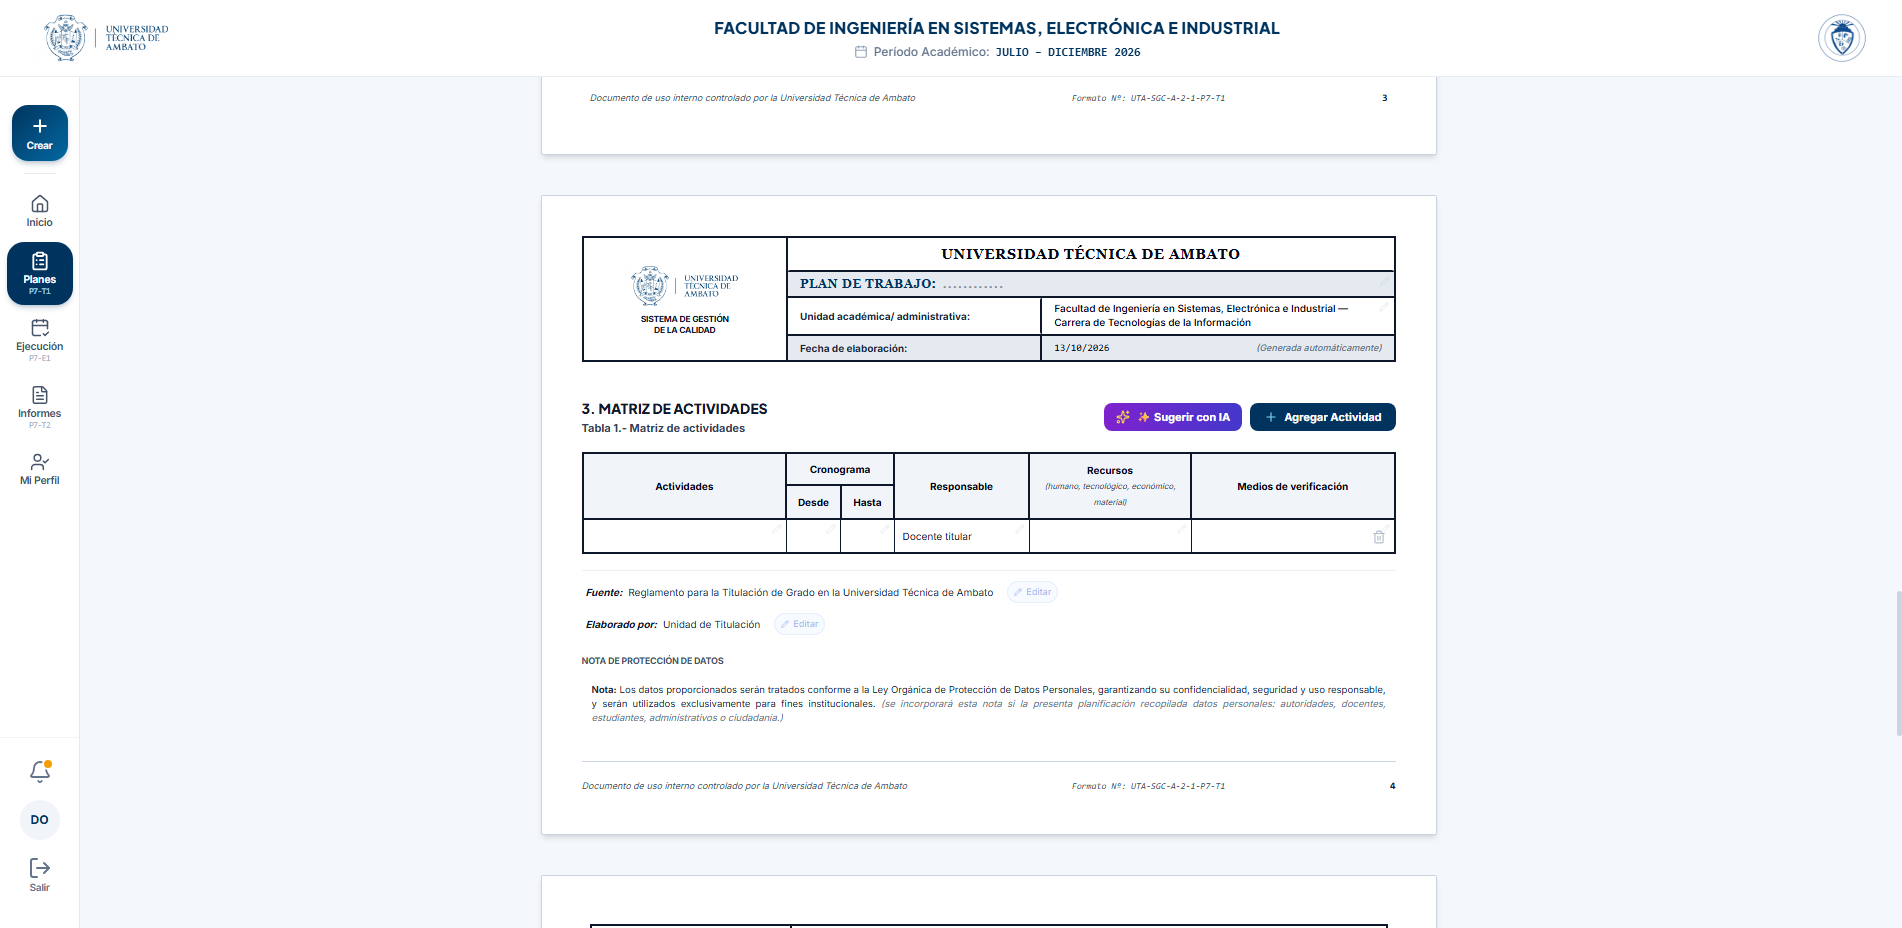
\includegraphics[width=0.88\textwidth,height=5.8cm,keepaspectratio]{images/sige_matriz_dinamica_actividades.png}
    \caption{Captura Real de la Demostración de la Matriz Dinámica durante la Sesión de Hito 4.}
    \label{fig:hito4_demo1}
\end{figure}
\FloatBarrier

\begin{figure}[H]
    \centering
    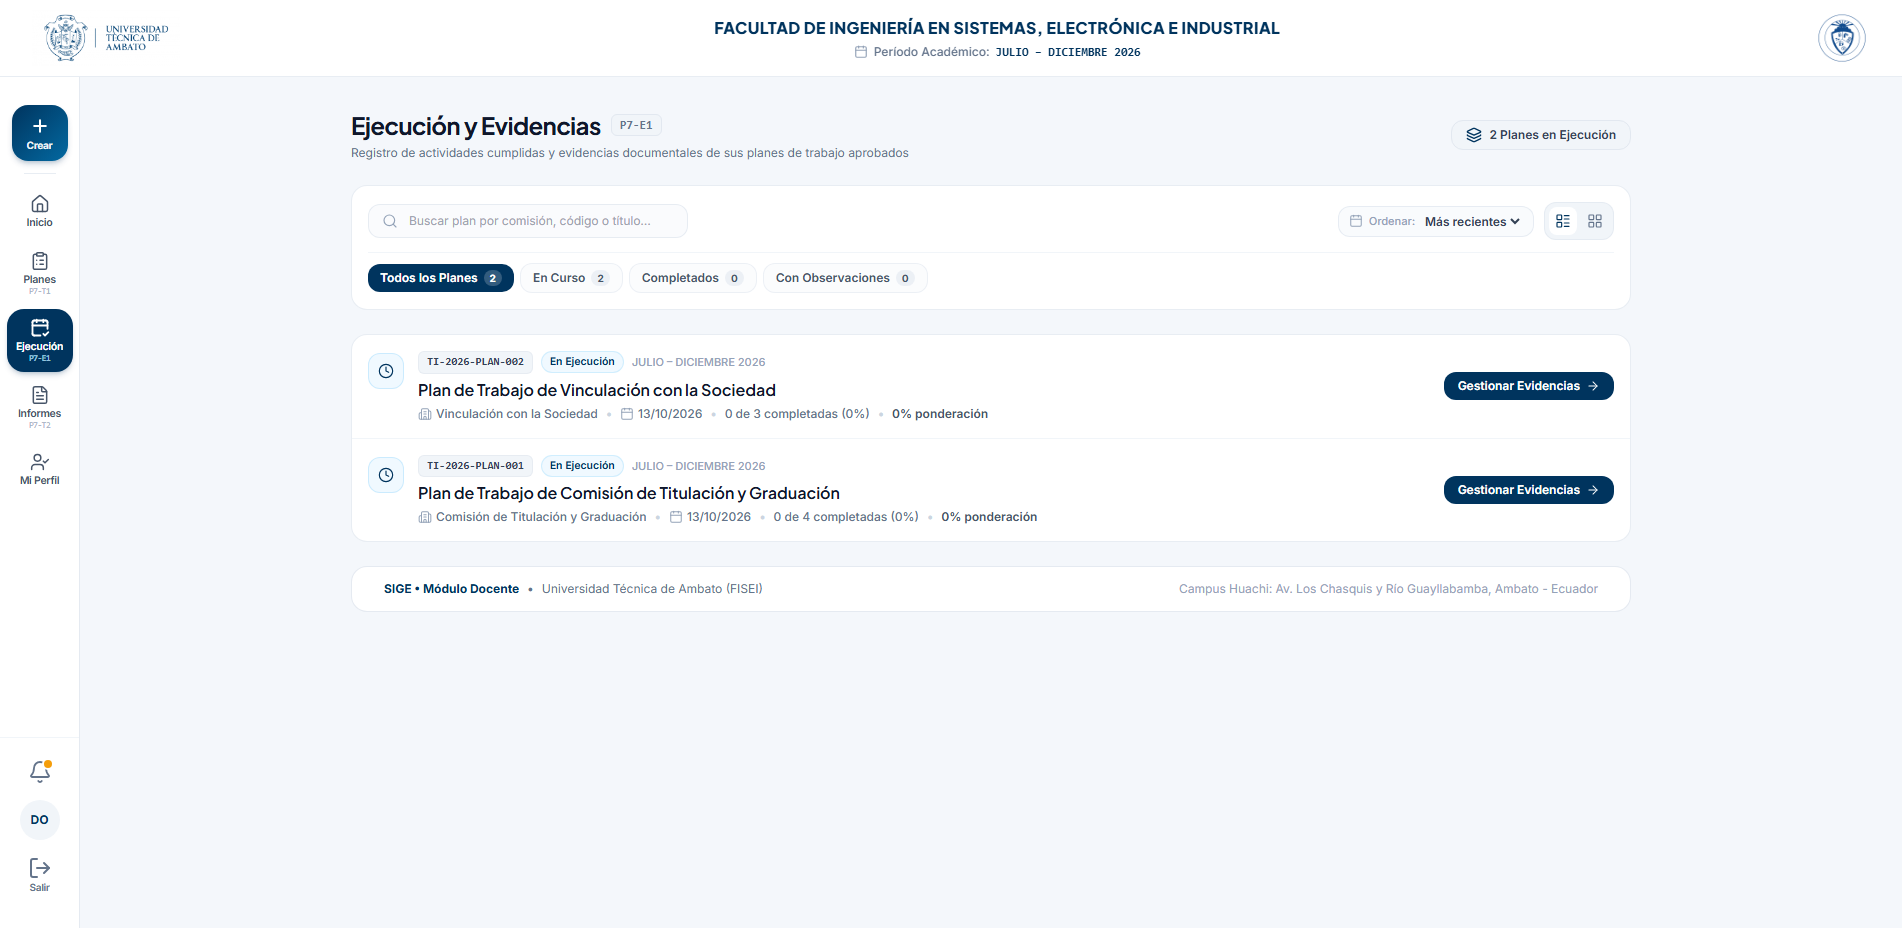
\includegraphics[width=0.88\textwidth,height=5.6cm,keepaspectratio]{images/sige_seguimiento_evidencias.png}
    \caption{Captura Real de la Verificación de Evidencias MinIO durante la Demostración de Hito 4.}
    \label{fig:hito4_demo2}
\end{figure}
\FloatBarrier

\section{Descripción de actividades}
\subsection{Matriz de Aceptación de Historias de Usuario del Sprint 3}
\begin{table}[H]
\centering
\small
\renewcommand{\arraystretch}{1.2}
\begin{tabularx}{\textwidth}{|c|>{\raggedright\arraybackslash\bfseries}m{3.2cm}|X|c|c|}
\hline
\rowcolor{tableheader}
\textbf{Código} & \textbf{Historia de Usuario} & \textbf{Criterio de Aceptación Evaluado} & \textbf{Resultado} & \textbf{Estado} \\
\hline
US-11 & Matriz Dinámica 100\% & Sumatoria reactiva al 100.00\% y selector de 16 semanas. & 100\% & Aprobada \\
\hline
US-12 & Validation Gates & Bloqueo en Express v5 ante horas $\ne 40$ o faltantes de evidencia. & 100\% & Aprobada \\
\hline
US-13 & Carga S3 en MinIO & Almacenamiento seguro de archivos PDF en bucket privado. & 100\% & Aprobada \\
\hline
US-14 & Integridad SHA-256 & Cómputo e inserción de hash de 64 caracteres en base de datos. & 100\% & Aprobada \\
\hline
US-15 & URLs Prefirmadas & Visualización de respaldos con enlace temporal de 15 min. & 100\% & Aprobada \\
\hline
\end{tabularx}
\caption{Matriz oficial de aceptación del incremento funcional del Sprint 3.}
\label{tab:sprint3_matrix}
\end{table}

\subsection{Métricas de Cumplimiento Acumulado del Proyecto al Hito 4}
\begin{table}[H]
\centering
\small
\renewcommand{\arraystretch}{1.2}
\begin{tabularx}{\textwidth}{|>{\bfseries}m{3.8cm}|c|c|X|}
\hline
\rowcolor{tableheader}
\textbf{Indicador de Proyecto} & \textbf{Planificado} & \textbf{Ejecutado} & \textbf{Estado Actual del Proyecto} \\
\hline
Horas Invertidas Sprint 3 & 96 h & 96 h & Avance exacto según cronograma Gantt. \\
\hline
Horas Acumuladas Fase 3 & 256 h & 256 h & 12 de 16 tareas de Fase 3 completadas ($75\%$). \\
\hline
Schedule Performance Index & 1.00 & 1.00 & Cero retrasos en hitos de entrega. \\
\hline
\end{tabularx}
\caption{Métricas acumuladas de avance del proyecto al Hito 4.}
\end{table}

\subsection{Línea Base del Cronograma del Proyecto SIGE al Cierre del Hito 4}
A la fecha de corte del Hito 4 (02 de octubre de 2026), se certifica la culminación de 3 de los 4 Sprints de desarrollo, restando únicamente el Sprint final de integración de firmas y exportación:

\begin{table}[H]
\centering
\small
\renewcommand{\arraystretch}{1.2}
\begin{tabularx}{\textwidth}{|c|>{\raggedright\arraybackslash\bfseries}m{3.2cm}|m{2.5cm}|c|c|c|}
\hline
\rowcolor{tableheader}
\textbf{Fase / Sprint} & \textbf{Denominación Oficial} & \textbf{Período Planificado} & \textbf{Tareas} & \textbf{Horas Netas} & \textbf{Estado al Hito 4} \\
\hline
\textbf{Fase 1} & Análisis y Planificación & 12 ago -- 18 ago 2026 & 8 & 192 h & \textbf{100\% CUMPLIDO (Aprobado)} \\
\hline
\textbf{Fase 2} & Diseño y Arquitectura & 19 ago -- 31 ago 2026 & 7 & 192 h & \textbf{100\% CUMPLIDO (Aprobado)} \\
\hline
\textbf{F3 - Sprints 1 a 3} & Base, Wizard y Matriz & 01 sep -- 02 oct 2026 & 12 & 300 h & \textbf{100\% CUMPLIDO (Aprobado)} \\
\hline
\textbf{F3 - Sprint 4} & Revisión, Firmas y NLP & 05 oct -- 12 oct 2026 & 4 & 100 h & \textit{0\% PROGRAMADO (Siguiente)} \\
\hline
\textbf{Fase 4} & Pruebas y Cierre Formal & 12 oct -- 13 oct 2026 & 3 & 48 h & \textit{0\% PROGRAMADO (Octubre)} \\
\hline
\multicolumn{3}{|r|}{\textbf{TOTAL GENERAL DEL PROYECTO:}} & \textbf{34} & \textbf{832 h} & \textbf{Avance Global: 82.2\%} \\
\hline
\end{tabularx}
\caption{Línea Base del Cronograma del Proyecto SIGE al cierre del Hito 4 (02 de octubre de 2026).}
\label{tab:linea_base_hito4}
\end{table}

\section{Firmas de Responsabilidad}

\noindent
\renewcommand{\arraystretch}{1.2}
\begin{tabularx}{\textwidth}{|>{\raggedright\arraybackslash}m{2.9cm}|>{\raggedright\arraybackslash}X|>{\centering\arraybackslash}m{4.6cm}|>{\centering\arraybackslash}m{2.3cm}|}
    \hline
    \rowcolor{tableheader}
    \textbf{ACCIÓN} & \textbf{NOMBRE Y CARGO} & \textbf{FIRMA} & \textbf{FECHA} \\
    \hline
    \textbf{Elaborado por:} & Heidi Villavicencio\newline Analista de Calidad / UI-UX & \parbox[c]{4.4cm}{\centering\vspace{4pt}
\includegraphics[height=1.5cm,width=4.0cm,keepaspectratio]{images/firma_heidi.png}\vspace{4pt}} & 02/10/2026 \\
    \hline
    \textbf{Revisado por:} & Steeven Toala\newline Líder de Proyecto / Arquitecto & \parbox[c]{4.4cm}{\centering\vspace{4pt}
\includegraphics[height=1.5cm,width=4.0cm,keepaspectratio]{images/firma_steveen.png}\vspace{4pt}} & 02/10/2026 \\
    \hline
    \textbf{Aprobado por:} & Ing. Paulo Torres, Mg.\newline Docente Evaluador -- Gestión Proyectos & \parbox[c]{4.4cm}{\centering\vspace{8pt}\textbf{\textcolor{gray!80}{\scriptsize [ PENDIENTE DE APROBACIÓN ]}}\vspace{8pt}} & \textbf{\textcolor{gray!90}{Pendiente}} \\
    \hline
\end{tabularx}

\vspace{0.4cm}

\section{Control de Cambios}

\noindent
\renewcommand{\arraystretch}{1.2}
\begin{tabularx}{\textwidth}{|>{\hsize=0.45\hsize\centering\arraybackslash}X|>{\hsize=1.55\hsize\raggedright\arraybackslash}X|>{\hsize=1.2\hsize\raggedright\arraybackslash}X|>{\hsize=0.8\hsize\centering\arraybackslash}X|}
    \hline
    \rowcolor{tableheader}
    \textbf{Versión} & \textbf{Descripción del cambio} & \textbf{Responsable del cambio} & \textbf{Fecha de aprobación} \\
    \hline
    1.0 & Emisión inicial del entregable según EDT del Tablero Trello & Equipo de Proyecto SIGE & 02/10/2026 \\
    \hline
\end{tabularx}

\vspace{0.4cm}

\section{Anexos}

\subsection*{Anexo 1: Ficha Técnica de la Tarea EDT 3.12 en el Tablero Trello}
\begin{table}[H]
\centering
\small
\renewcommand{\arraystretch}{1.2}
\begin{tabularx}{\textwidth}{|>{\bfseries}m{3.5cm}|X|}
\hline
\rowcolor{tableheader}
\textbf{Parámetro EDT} & \textbf{Detalle Oficial del Tablero Trello} \\
\hline
Código de Tarea & EDT 3.12 \\
\hline
Nombre de la Tarjeta & HITO 4: Sprint 3 Review: Matriz Dinámica y Evidencias MinIO \\
\hline
Fase Correspondiente & FASE 3. IMPLEMENTACIÓN Y DESARROLLO \\
\hline
Período de Ejecución & 01 de octubre al 02 de octubre de 2026 (2 días laborables) \\
\hline
Horas Asignadas & 16 horas hombre netas \\
\hline
Responsables Técnicos & Steeven Toala (ST), Andrea Vásquez (AV), Nixon Hurtado (NH), Heidi Villavicencio (HV) \\
\hline
Entregable Oficial & Demostración funcional de matriz con evidencias MinIO \\
\hline
Estado en el Tablero & 100\% Completado y Aprobado Formalmente \\
\hline
\end{tabularx}
\caption{Ficha técnica de la tarea EDT 3.12 en el Tablero Trello.}
\end{table}

\subsection*{Anexo 2: Acta Formal de Aprobación del Sprint 3 (Hito 4)}
\begin{table}[H]
\centering
\footnotesize
\renewcommand{\arraystretch}{1.15}
\begin{tabularx}{\textwidth}{|m{3.0cm}|X|}
\hline
\rowcolor{tableheader}
\multicolumn{2}{|c|}{\textbf{ACTA INSTITUCIONAL DE CIERRE DE SPRINT 3 -- SISTEMA SIGE}} \\
\hline
\textbf{Fecha de Sesión:} & 02 de octubre de 2026 \\
\hline
\textbf{Participantes:} & Steeven Toala (Líder Técnico), Andrea Vásquez (Frontend), Nixon Hurtado (Backend), Heidi Villavicencio (Calidad), Ing. Paulo Torres (Docente Evaluador). \\
\hline
\textbf{Resolución:} & Tras presenciar la demostración de recálculo aritmético instantáneo de la Matriz Dinámica al 100\%, el bloqueo preventivo de las Validation Gates y la persistencia de evidencias en MinIO S3 con hashes SHA-256, el Docente Evaluador declara APROBADO por unanimidad el Hito 4 y autoriza el inicio del Sprint 4 enfocado en Revisión Colegiada, Corrección Ortográfica y Exportación Oficial. \\
\hline
\end{tabularx}
\caption{Acta oficial de aprobación de Hito 4.}
\end{table}

\subsection*{Anexo 3: Lista de Chequeo y Criterios de Aceptación Institucional (SGC ISO 9001:2015)}
\begin{table}[H]
\centering
\footnotesize
\renewcommand{\arraystretch}{1.15}
\begin{tabularx}{\textwidth}{|m{3.2cm}|X|c|c|}
\hline
\rowcolor{tableheader}
\textbf{Criterio de Calidad SGC} & \textbf{Mecanismo de Verificación Técnica} & \textbf{Conformidad} & \textbf{Responsable} \\
\hline
Cumplimiento Sprint 3 & Historias de usuario US-11 a US-16 probadas y aceptadas al 100\% & 100\% CONFORME & Steeven Toala \\
\hline
Integración de Evidencias & Matriz dinámica y carga de archivos en MinIO operando con éxito & 100\% CONFORME & Heidi Villavicencio \\
\hline
Rendimiento del Cronograma & 100 horas netas ejecutadas en el Sprint 3 con índice SPI = 1.00 & 100\% CONFORME & Nixon Hurtado \\
\hline
Aprobación Colegiada & Acta formal de cierre de Hito 4 firmada por el Docente Evaluador & 100\% CONFORME & Ing. Paulo Torres \\
\hline
\end{tabularx}
\caption{Lista de verificación y control de calidad institucional del entregable 3.12.}
\end{table}


\end{document}
